\chapter{Launch Phase}
An initial analysis of the final system is made in order to estimate the development time it takes to develop the system. When knowing the development time of a product, this can be translated into an estimation of the total development cost. In the launch phase, everything not concerning the realization phase of the system have to be considered, in order to make a good time estimation. The black box which it will all ends up with have been defined in the Pre-Project, now one layer is pilled of the box at a time, which is done in the next 3 sections. Before digging in to the realization phase a detailed development plan for the product is then defined. 
%%%%%%%%%%%%%%%%%%%%%%%%%%%%%%%%%%%%%%%%%%%%%%%%%%%%%%%%%%
%%%%%%%%%%%%%%%%%%%%%%%%%%%%%%%%%%%%%%%%%%%%%%%%%%%%%%%%%%
\section{General Analysis}
In the general analysis section the requirement is found and tests to check if these requirements have been fulfilled created. Overall function blocks for the system are drawn, different ways of interacting with the system should be defined together with the design of the final product.
 
%%%%%%%%%%%%%%%%%%%%%%%%%%%%%%%%%%%%%%%%%%%%%%%%%%%%%%%%%%
\subsection{Requirement Analysis}
From the teachers wiki \footnote{http://teachers.ede.hih.au.dk/index.php/Main\_Page} requirements have been found and listed together with the requirements defined by the customer. The requirements have been divided in groups:
\begin{itemize}
	\item Functional Requirements ("system shall do 'requirement' ")
	\item Non-functional Requirements ("system shall be 'requirement' ")
	\item Behavioural Requirements ("how the system shall react")
	\item Performance Requirements ("how well does it have to be done")
\end{itemize}
Common requirements for the energy system can be found on the E10 wiki \footnote{http://e10.ede.hih.au.dk/index.php/Common\_Requirements}
% Functional Table
\begin{table}[H]
	\begin{tabular} [b] {| p{1.2cm} |  p{3.5cm} | p{11.3cm} |}
	\hline
	\textbf{ID} & \textbf{Requirement} & \textbf{Description} \\\hline
		F-1 & Communication 	&  \\ \hline
		F-1.1 & Web Server 		& The hub shall be able to put data on a web-server. \\ \hline
		F-1.2 & System 		& The hub shall be able to communicate with a connected module through power line communication. \\ \hline
		F-1.2.1 & Protocol 		& The Power Line Communication shall be done according to the common protocol (see appendix: Protocol)\\ \hline
		F-2 & Routing 			&  \\ \hline
		F-2.1 & Direction		& When a module is connected the system shall automatically find out if it is an producer-, storage- or consumer module.\\ \hline
		F-2.2 & Consumer		& Only allowed to take energy from the system. \\ \hline
		F-2.3 & Producers 		& Only allowed to give energy to the system. \\ \hline
		F-2.4 & Storage 		& Must acts either as a consumer or a producer (can be changed dynamically). \\ \hline
	\end{tabular}
	\caption{Functional: System shall do...}
\end{table}
% Non-Function Table
\begin{table}[H]
	\begin{tabular} [b] {| p{1.2cm} |  p{3.5cm} | p{11.3cm} |}
	\hline
	\textbf{ID} & \textbf{Requirement} & \textbf{Description} \\\hline
		NF-1 & User Interface 	&  \\ \hline
		NF-1.1 & Web Interface 	& Maximum 2 click to go where you want on the website. \\ \hline
		NF-1.2 & HW Interface	& Able to connect 10 modules to the hub. \\ \hline
		NF-1.3 & HW Interface	& A locker shall be unlocked to access the physical hw. \\ \hline
		NF-1.4 & HW interface	& An Emergency stop shall be visible on the hub and shall shut down the system if pushed. \\ \hline
		NF-1.5 & HW Interface	& 1 start button for the hub. 10 buttons to each start a module. \\ \hline
		NF-2 & Electrical 		&  \\ \hline
		NF-2.1 & Voltage 		& The input and output ports must work in the range 30V +/-  10\%.\\ \hline
		NF-2.2 & Current 		& The maximum current on each port is defined to maximum 30 Amperes. \\ \hline
	\end{tabular}
	\caption{Non-Function: System shall be...}
\end{table}
% Perfomance Table
\begin{table}[H]
	\begin{tabular} [b] {| p{1.2cm} |  p{3.5cm} | p{11.3cm} |}
	\hline
		\textbf{ID} & \textbf{Requirement} & \textbf{Description} \\\hline
		P-1 & Hardware 		&  \\ \hline
		P-1.1 & Housing 		& The housing have to be water-proof, to not harm the system.\\ \hline
	\end{tabular}
	\caption{Performance: How well does it have to be done...}
\end{table}
% Behavioural Table
\begin{table}[H]
	\begin{tabular} [b] {| p{1.2cm} |  p{3.5cm} | p{11.3cm} |}
	\hline
	\textbf{ID} & \textbf{Requirement} & \textbf{Description} \\ \hline
		B-1 	&  Status 			&  \\ \hline
		B-1.1 & Web Interface	& Warnings are posted in the web interface. \\\hline
		B-1.2 & Physical		& 1 diode showing when a module is off and one showing when it is on.\\ \hline
		B-1.3 & Report			& An e-mail is sent to the defined user if an error occurs. \\\hline
		B-2 & Energy Control	&  \\\hline
		B-2.1 & Over-production	& Overproduced energy is wasted in a dummy load connected to the hub. \\\hline
		B-2.2 & Over-production	& If two or more producers are connected and one can be without, it is stopped.  \\\hline
		B-2.2 & Under-production	& If there is no overproduction (dummy load is turned off), the grid is connected to the power line in case the producers cannot produce enough energy. \\\hline
		B-3 & Errors	 		& Humidity and Temperature sensor will be placed inside the system housing. \\\hline
		B-3.1 & Humidity		& If the humidity is above the maximum level 70\%, the system shuts down. \\\hline
		B-3.2 & Temperature High& If the temperature is higher than 55 degrees,  the system shuts down.\\\hline
		B-3.2 & Temperature Low & If the temperature is below 0 degrees, the system shuts down\\\hline
	\end{tabular}
	\caption{Behavioural: How the system shall react...}
\end{table}
%%%%%%%%%%%%%%%%%%%%%%%%%%%%%%%%%%%%%%%%%%%%%%%%%%%%%%%%%%
\subsection{Requirement tests}
In order to verify that the requirements have been fulfilled, tests should be done. Most of the tests should be done together with the customer in order to get his acceptance that he received what he ordered. 
\\After a test has finished, a binary grade will be given (pass / fail), together with a comment telling how the test went: where it was done, with whom and when it was done.
\\[0.2cm]\textbf{Test of the Functional Requirements}
\begin{table}[H]
	\begin{tabular} [b] {| p{1.2cm} |  p{9.3cm} | p{1.2cm} | p{3.8cm} |}
	\hline
	\textbf{ID} & \textbf{Test Description} & \textbf{Grade} & \textbf{Comment} \\\hline
		F-1.1 	& Check if the parameters on the website is updating. The easiest parameter to validate is the uptime of the system. Check the website with half a minute in between and verify that the parameter has been updated. 	&	&\\ \hline
		F-1.2 	& Connect a module to the hub, by connecting the module to the hubs power line (plugs on the back of the hub). If the module respond to a ping signal send from the hub, the two modules are communicating through power line. The response of the ping can be seen by using an oscilloscope and simply analyzing the packages on the power line according to the protocol. 	&	&\\ \hline
		F-1.2.1 	& A test of the protocol is placed together with the description of it. This test is verified in corporation with the rest of the teams.	&	&\\ \hline
		F-2.1 	& Connect 3 modules: a producer, consumer and a storage device one at the time. Verify that the hub has correctly read the modules by checking connected modules on the website.	&	&\\ \hline
		F-2.2 	& Connect a consumer to the hub. Verify that the current flow is going to the consumer.	&	&\\ \hline
		F-2.3 	& Connect a producer to the hub. Verify that the current flow is going to the hub.	&	&\\ \hline
		F-2.4 	& Connect a storage device together with a producer. Verify that the current flow is only going to the storage device. Turn of the producing module and connect a consumer (note that the storage device shall have some energy stored). Verify that the current flow is only going from the storage device.	&	&\\ \hline
	\end{tabular}
	\caption{Functional requirement test}
\end{table}
\textbf{Test of the Non-Functional Requirements}
\begin{table}[H]
	\begin{tabular} [b] {| p{1.2cm} |  p{9.3cm} | p{1.2cm} | p{3.8cm} |}
	\hline
	\textbf{ID} & \textbf{Test Description} & \textbf{Grade} & \textbf{Comment} \\\hline
		NF-1	.1	& The user is asked to go through some simple steps. See production of a connected module. Login, start a module, stop a module. Check alternative energy production (money, CO2, bulbs).	Together with the user it is accepted that there is maximum 2 clicks to find a  certain thing on the website. &	&\\ \hline
		NF-1	.2	& Check if there are 10 module connectors on the back of the hub module. Verify that all connectors work by connecting a module to one input at the time and check that a red diode for the module input turns on. 	&	&\\ \hline
		NF-1	.3	& Together with the user it is verified that he cannot control the front interface without unlocking the system with a key. 	&	&\\ \hline
		NF-1	.4	& Check that an emergency button is visible on the hub (the user decides if it is visible enough). The button is checked by getting the system up and running and pressing the emergency button. The system shall now shut down.	&	&\\ \hline
		NF-1	.5	& It is visible inspected that 11 start buttons can be found on the physical hub interface	&	&\\ \hline
		NF-2.1	& The voltage found on the power line is handled in the modules. Test can be found in the common requirement document. However the power line is measured with a voltmeter (without any modules on, only the grid) and shall be in the range 27-33V	&	&\\ \hline
		NF-2.2	& The maximum current given or taken is handled in the modules. Test can be found in the common requirement document.	&	&\\ \hline
	\end{tabular}
	\caption{Non-Functional requirement test}
\end{table}
\textbf{Test of the Performance Requirements}
\begin{table}[H]
	\begin{tabular} [b] {| p{1.2cm} |  p{9.3cm} | p{1.2cm} | p{3.8cm} |}
	\hline
	\textbf{ID} & \textbf{Test Description} & \textbf{Grade} & \textbf{Comment} \\\hline
		P-1.1	& Inspect the housing together with the customer, while water is being dumped on the roof and the sites of it &	&\\ \hline
	\end{tabular}
	\caption{Performance requirement test}
\end{table}
\textbf{Test of the Behavioural Requirements}
\begin{table}[H]
	\begin{tabular} [b] {| p{1.2cm} |  p{9.3cm} | p{1.2cm} | p{3.8cm} |}
	\hline
	\textbf{ID} & \textbf{Test Description} & \textbf{Grade} & \textbf{Comment} \\\hline
		B-1.1	& A module is connected to the hub, depending on the available module: -Battery module: disconnect all batteries (no batteries) -Wind module: turn the turbine away from the wind (low wind) Photo-cell module: Cover the cells (low sun). If one of the above states are done, a warning message should be posted on the website	&	&\\ \hline
		B-1.2	& Check that two diodes are shown next to a module start button (one red and one green). Connect a module, now check that the red diode turns on. Go to the website and turn on the module, check that the green diode turns on.	&	&\\ \hline
		B-1.3	& Connect a module to the hub and start it. When the status of the module is running (see on the website), the module is unplugged. Now check the mail box of the user and verify that a mail has been received from the energy system.	&	&\\ \hline
		B-2.1	& A dummy load and a producing module is connected to the system. As no consumers is connected, the system is overproducing. The current flow to the dummy load is measured. If the current flowing to the dummy load is the same as the one coming from the producer (maximum -10\%), the test is valid.	&	&\\ \hline
		B-2.2	& A dummy load and a producing module is connected to the system. As no consumers is connected, the system is overproducing. A variable consuming module is now connected. The resistance in the consuming module is decreased (increasing load). The current flow to the dummy load shall now fall. When no current is flowing to the dummy load, it shall be observed that the grid is connected. This is done by increasing the load of the consuming module and measuring the current flow from the grid.	&	&\\ \hline
		B-3.1	& A water boiler is placed below the humidity censor. A humidity interment is placed next to the hubs humidity sensor. The hubs reaction when the humidity comes above 70\% is observed. If the hub shuts off, the test has been successful.	&	&\\ \hline
		B-3.2	& If a climate cabinet is available, the heat tests will be performed there, otherwise a heating gun will be used to increase the temperature. A temperature instrument is placed next to the hubs temperature sensor. The hubs reaction when the temperature comes above 55deg is observed. If the hub shuts off, the test has been successful.	&	&\\ \hline
		B-3.3	& If a climate cabinet is available, the heat tests will be performed there, otherwise cooling spray will be used to decrease the temperature. A temperature instrument is placed next to the hubs temperature sensor. The hubs reaction when the temperature comes below 0deg is observed. If the hub shuts off, the test has been successful.	&	&\\ \hline
	\end{tabular}
	\caption{Behavioural requirement test}
\end{table}


%%%%%%%%%%%%%%%%%%%%%%%%%%%%%%%%%%%%%%%%%%%%%%%%%%%%%%%%%%
%%%%%%%%%%%%%%%%%%%%%%%%%%%%%%%%%%%%%%%%%%%%%%%%%%%%%%%%%%
\newpage
\subsection{Problem Domain Analysis}
Everything that should be controlled by the system-to-be will be defined here. 
%%%%%%%%%%%%%%%%%%%%%%%%%%%%%%%%%%%%%%%%%%%%%%%%%%%%%%%%%%
\subsubsection{Block Diagram:}
Block diagram of the hub. Showing all the things that the hub should interface with.
	\begin{figure}[H]
		\begin{centering}
			 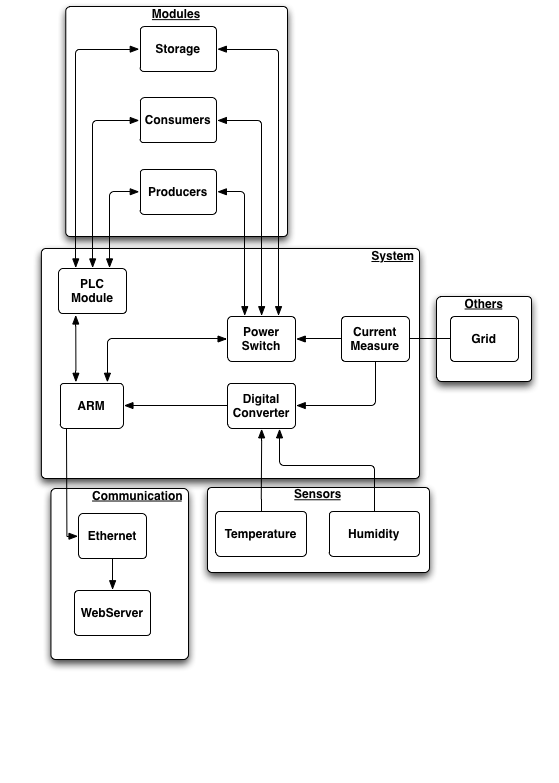
\includegraphics[width=0.78\textwidth]{images/block_diagram.png}
			\caption{Block diagram}
	 	\end{centering}
	\end{figure}

%%%%%%%%%%%%%%%%%%%%%%%%%%%%%%%%%%%%%%%%%%%%%%%%%%%%%%%%%%
\subsubsection{Block Diagram: Candidates in the system}
\begin{itemize}
	\item \textbf{Power Switch:} Part of the hub that powers the connected modules on or off.
	\item \textbf{Consumers} Modules that consumes power (e.g. light, washing machine, electric car)
	\item \textbf{Producers:} Modules that delivers energy to the hub (e.g. Wind-turbine, photovoltaic-cells)
	\item \textbf{Storage:} Modules that both consumes when the system over produces and "produces" (gives energy to the consumers) when needed (e.g. battery, air compressor). 
	\item \textbf{Grid:} The grid is used to start up the whole system. It is also used if producing modules does not produce enough energy to the consumers.
	\item \textbf{Current Sensor:} Unit that measures the current taken from the grid. To calculate the amount of green energy produced.
	\item \textbf{Temperature:} Unit that measures the temperature where the system is placed. If the temperature is too high or low it might damage the hardware.
	\item \textbf{Humidity:} Unit that measures the humidity where the system is places. If the humidity is too high the hardware might be damaged.
	\item \textbf{Ethernet:} Unit that has connection to an internet database.
\end{itemize}

%%%%%%%%%%%%%%%%%%%%%%%%%%%%%%%%%%%%%%%%%%%%%%%%%%%%%%%%%%
\subsubsection{Block Diagram: Events in the system}
All candidates shown in the block diagram.
	\begin{itemize}
		\item TemperatureBelowLimit
		\item TemperatureAboveLimit
		\item HumidityAboveLimit
		\item CurrentMaxLimit
		\item CurrentMinLimit
		\item EnergyAboveLimit
		\item EnergyBelowLimit
		\item InitModule
		\item StartModule
		\item StopModule
		\item StandbyModule
		\item CreateModuleLogFile
		\item LoadModuleLogFile
		\item UpdateModuleLogFile
		\item UpdateServer
	\end{itemize}
\textbf{Table with all the above candidates and event combined:}
All the different events that can happen in a block or sent between blocks. 
	\begin{table}[H]
	\begin{tabular}{| r | c |c | c | c | c | c | c | c | c |}
	\hline
		~ & 					P SW & Cons. & Prod. & Storage & Grid & Curr Sens & Temp & Humi & Ether. \\ \hline
		TempBellowLimit 		& ~          & ~         & ~         & ~           & ~           & ~               & X      & ~ 	       & ~	\\ \hline
		TempAboveLimit 		& ~          & ~         & ~         & ~           & ~           & ~               & X      & ~ 	       & ~	\\ \hline
		HumidityAboveLimit	 	& ~          & ~         & ~         & ~           & ~           & ~               & ~      & X 	       & ~	\\ \hline
		InitModule 			& ~          & X         & X         & X           & ~           & ~              & ~      & ~ 	       & ~	\\ \hline
		StartModule 			& ~          & X         & X         & X           & X           & ~              & ~      & ~ 	       & ~	\\ \hline
		StopModule 			& ~          & X         & X         & X           & X           & ~              & ~      & ~ 	       & ~	\\ \hline
		StandbyModule 		& ~          & ~         & X         & X           & ~           & ~               & ~      & ~ 	       & ~	\\ \hline
		CurrentMaxLimit	 	& ~          & ~         & ~         & ~           & X           & X               & ~      & ~ 	       & ~	\\ \hline
		CurrentMinLimit	 	& ~          & ~         & ~         & ~           & X           & X               & ~      & ~ 	       & ~	\\ \hline
		EnergyAboveLimit 		& ~          & ~         & X         & ~           & X           & ~               & ~      & ~ 	       & ~	\\ \hline
		EnergyBelowLimit 		& ~          & ~         & X         & ~           & X           & ~               & ~      & ~ 	       & ~	\\ \hline
		CreateModuleLogFile 	& ~          & ~         & X         & ~           & ~           & ~               & ~      & ~ 	       & ~	\\ \hline
		LoadModuleLogFile 	& ~          & ~         & X         & ~           & ~           & ~               & ~      & ~ 	       & ~	\\ \hline
		UpdateModuleLogFile 	& ~          & ~         & X         & ~           & ~           & ~               & ~      & ~ 	       & ~	\\ \hline
		UpdateServer			& ~          & ~         & ~         & ~           & ~           & ~               & ~      & ~ 	       & X	\\ \hline
	\end{tabular}
	\caption{Class diagram of all the hubs events and candidates.}
\end{table}
%%%%%%%%%%%%%%%%%%%%%%%%%%%%%%%%%%%%%%%%%%%%%%%%%%%%%%%%%%
\subsubsection{State Machine Diagram}
Digging deeper into the hub module, states in the different blocks is defined. 
\\[0.5cm] \underline{\textbf{Micro Processor (ARM) states:}}
\p \textbf{Description of the different states: }
	\\ After the initialization of all modules connected to the hub, the system is in  \textit{Idle Mode}.
	\p\textbf{Idle: } After initialization the hub goes into idle mode. The hub stays in idle mode until a start signal is given from the user (from the web or the physical hub interface). 
	\p\textbf{Run mode: }The system stays in Run Mode until an event happens, e.g. temperature or humidity reaches their limits, a new module is connected, a module should be removed, the system is over-/underproducing, the log should be updated etc.
	\p\textbf{Start: }Whenever a new module is connected it waits for the user to start the module from the web interface.
	\p\textbf{Stop: }To securely disconnect a module, the user must use the disconnect button (on web interface) to make sure all data is saved.
	\p\textbf{Shut down: }If the system finds itself in a critical condition (temperature, humidity, communication problems) it shutdown it's connected modules, tries to save all available data to the log. Then it sends an message (in form of e-mail) to the user, describing the problem, and the module powers off itself. 
	\p\textbf{Connect module: } The system checks if it has seen exactly that module before, if that is the case it updates variables from the database (uptime, production etc.). If the module is new for the system, it creates it in the database and gives it an unique id.
	\p\textbf{Warning: }Is sent if the system tries to set a submodule in start- or stop mode, but after a while it has not changed (timeout). After the timeout state, the system returns to run state.
	\begin{figure}[H]
		\begin{centering}
			 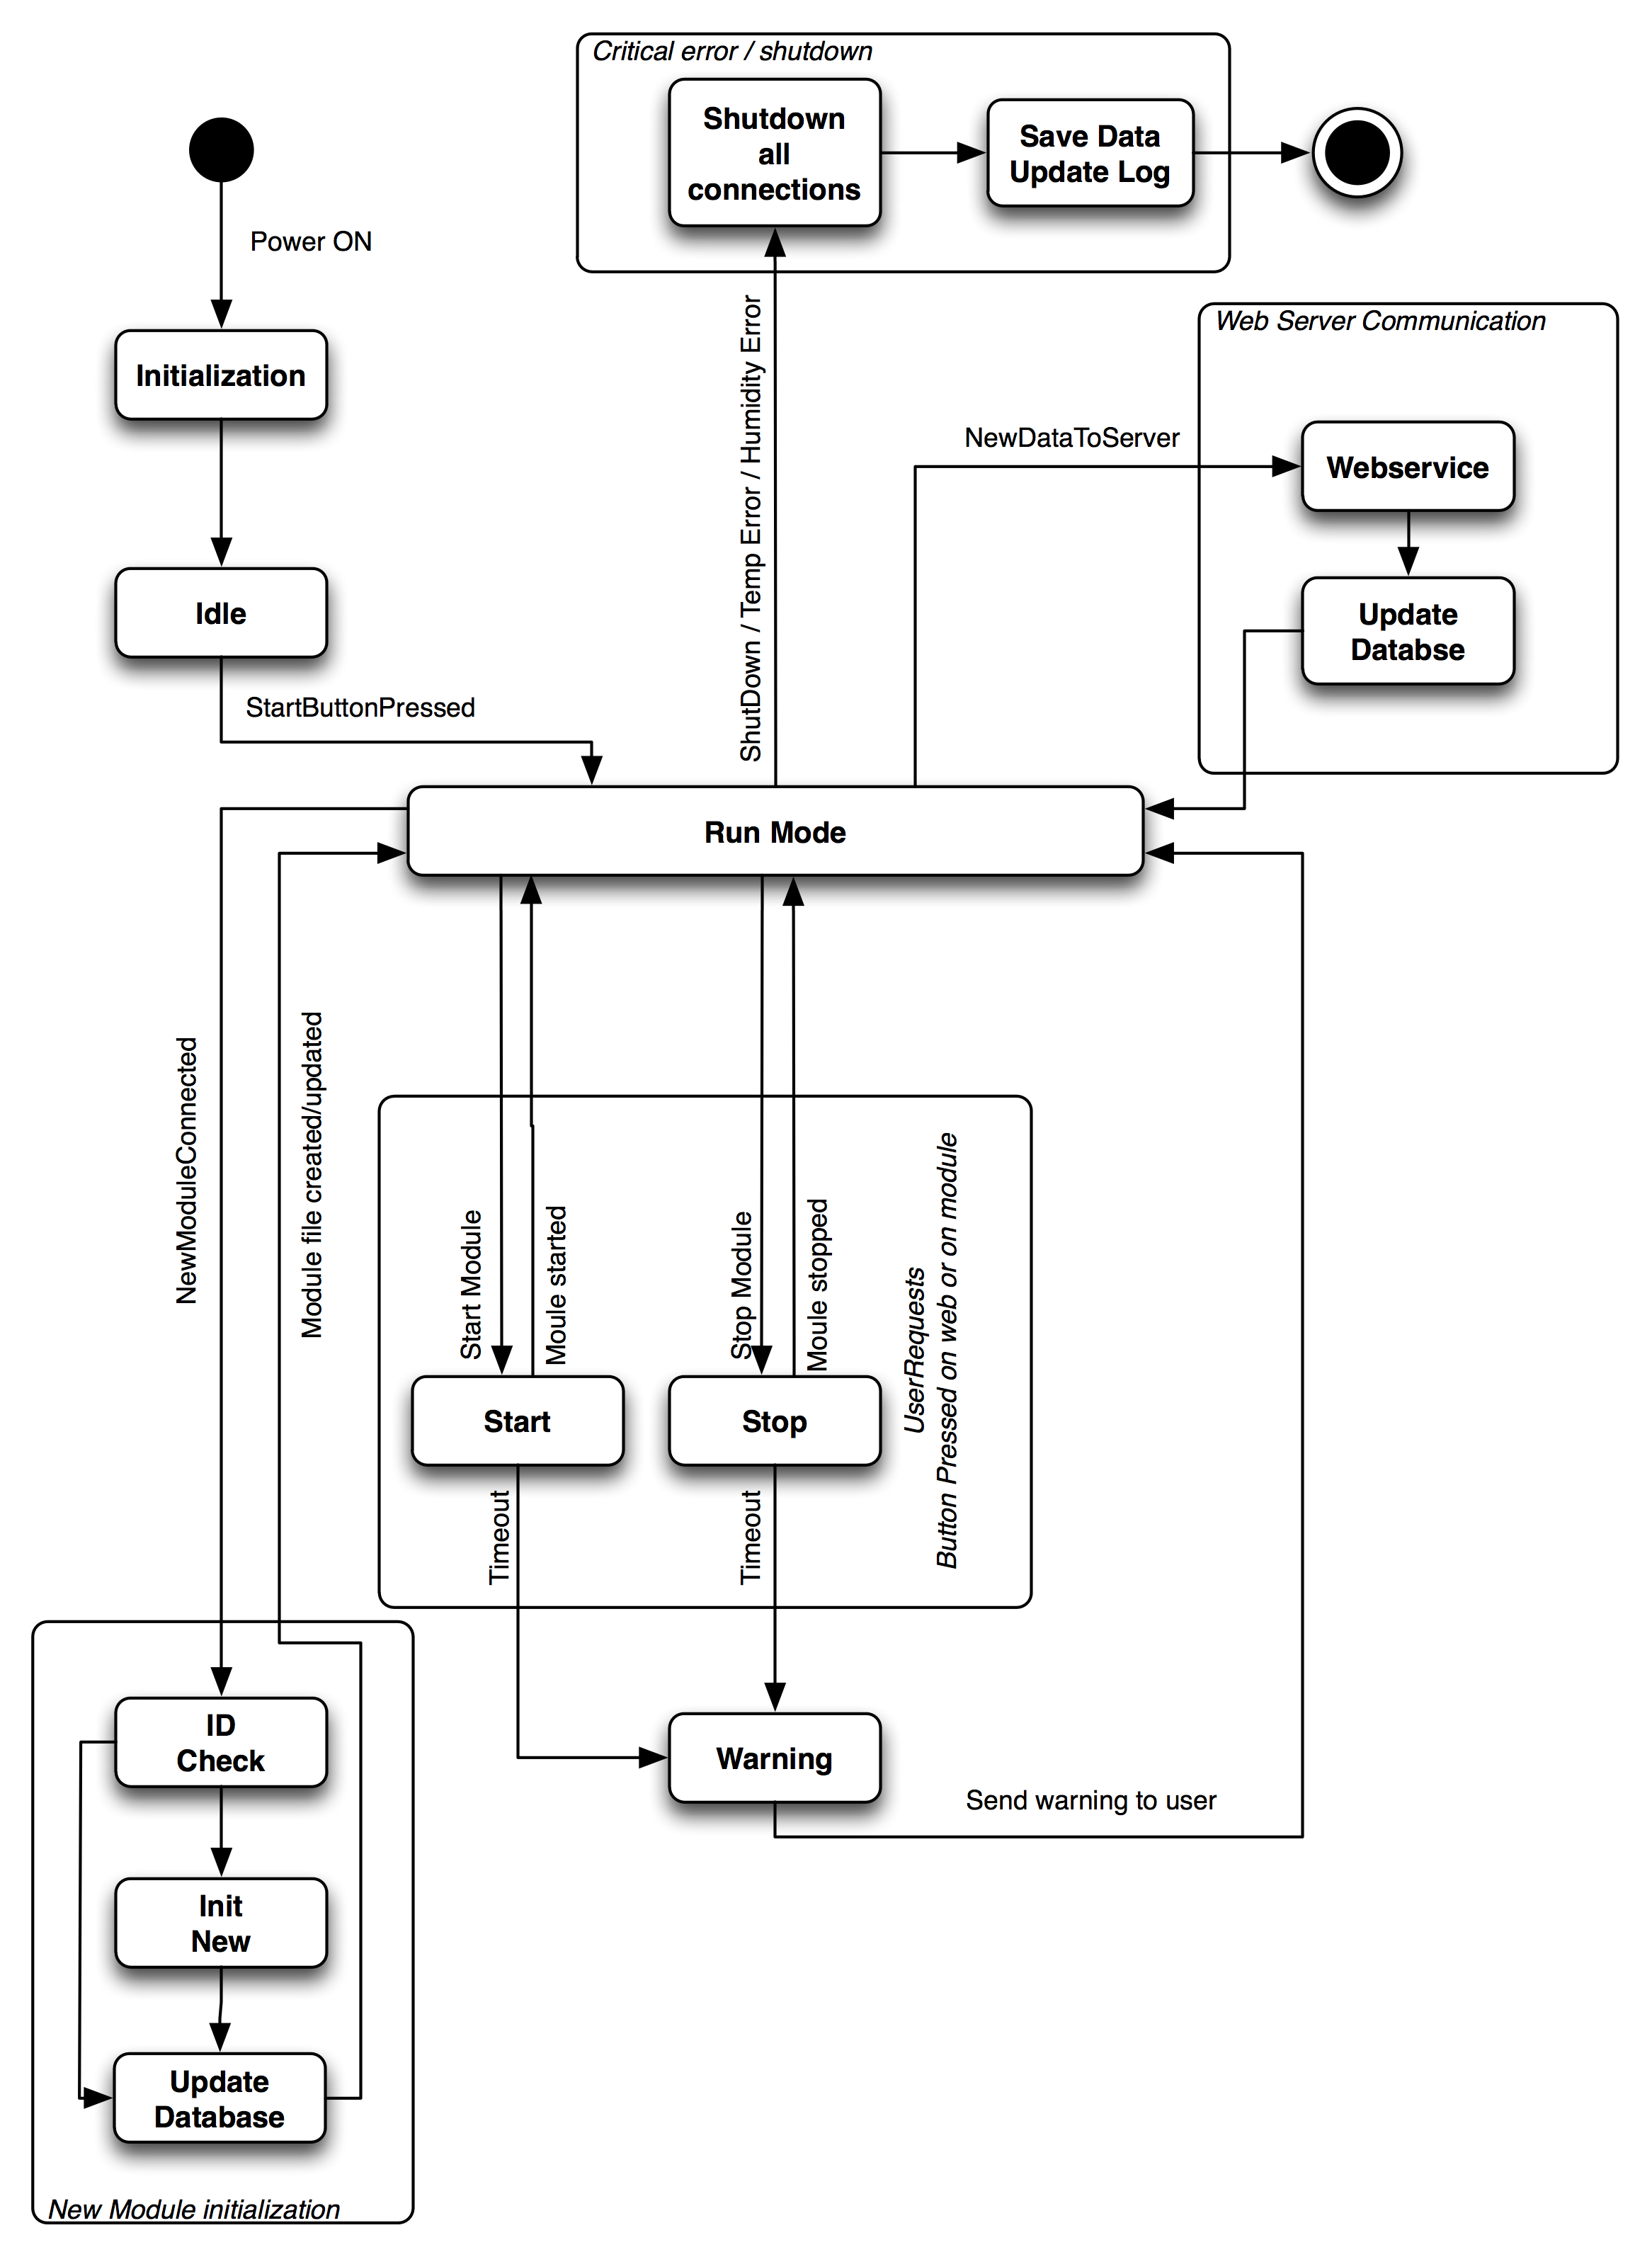
\includegraphics[width=0.9\textwidth]{images/statemachine.png}
		\caption{State Machine Diagram of the system}
	 	\end{centering}
	\end{figure}
	
\underline{\textbf{Web Server\:}}
\p \textbf{Description of the different states: }
	\textbf{Listening: }The system will listen the TCP / IP port until an event happens, e.g.  a new module is connected, a module should be removed, new data to the data base, user event from the web interface etc.
	\textbf{Webservices:} The web server will execute a PHP script, this will perform requests to the database and send start and stop commands to the hub.
	\p
	Webservices:
	\\- insertData: inserts new data to table ( module\_id, current, voltage, time of measure, status, efficiency  ) this are the data common to all modules.
	\\- selectData: show data to the user on the web page, this is a dynamic request.
	\\- clearData: resets database, by erasing the database and recreating and populating.
	\\- sendCmd ( Start / Stop / Cmd ): commands send from the web interface to control the system and different modules.
	\\- sendWarning: shows an warning in the web interface and the administrator receives a warning in the defined email address.
	

	\begin{figure}[H]
		\begin{centering}
			 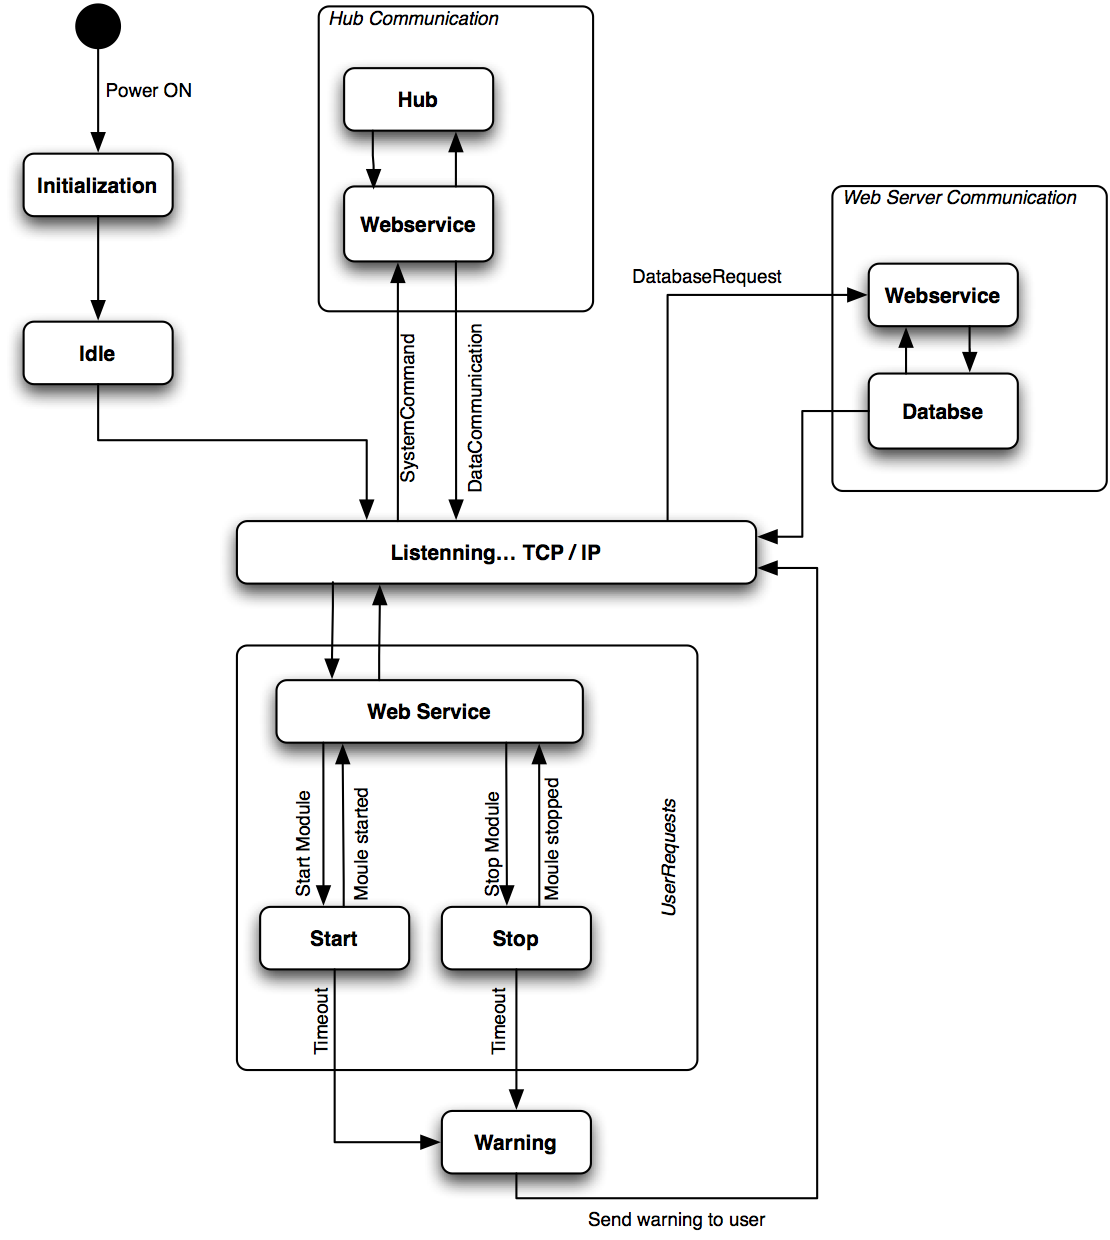
\includegraphics[width=0.9\textwidth]{images/state_web.png}
		\caption{State Machine Diagram of the Web Server}
	 	\end{centering}
	\end{figure}
	\p
	Database structure:
	\begin{figure}[H]
		\begin{centering}
			 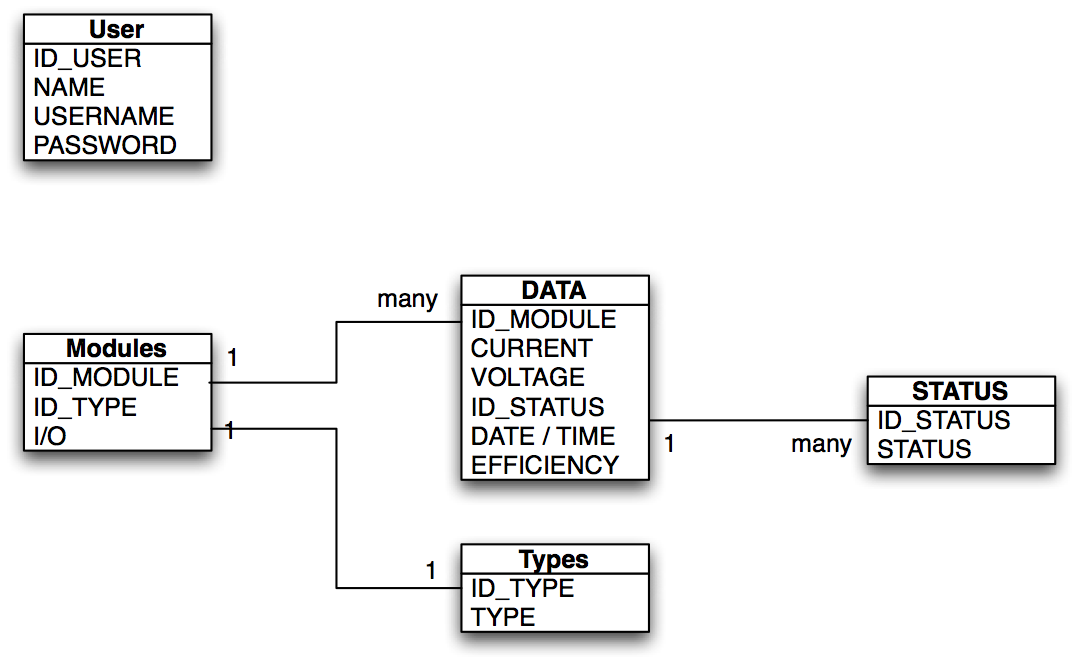
\includegraphics[width=0.9\textwidth]{images/db_prop.png}
		\caption{Database Structure}
	 	\end{centering}
	\end{figure}

%%%%%%%%%%%%%%%%%%%%%%%%%%%%%%%%%%%%%%%%%%%%%%%%%%%%%%%%%%
\subsection{Usage Domain Analysis}
A description of all the different users to the system and the actions each user are allowed to do.
\p \textbf{Web user - Log in}
\\\textit{Description: }An user with administrator privileges that can login to the web interface of the system. This user can manage the energy hub from a computer or mobile device via the web page and have permission to start and stop modules.
\p\textbf{Web user - Visitors}
\\\textit{Description: }	This visitor of the web interface can only see info and data on the web page for the system. This user do not have permission to manage anything.
\p\textbf{Hub}
\\\textit{Description: }	The Hub actor is the system, that have the ability to make action on its own, for example it have to be able to shutdown a module if an error occurs on that module.
\p\textbf{Engineer}
\\\textit{Description: }The engineer is any person with knowledge about how the system works on a technical level. This user is able to reprogram the whole system and have permission to everything.
\p\textbf{On system user}
\\\textit{Description: }	On system user is any user that go to the physical system and operates on it. This user is able to turn modules connected to the hub on or off.
\p
\p\textbf{Plug in module}
\\\textit{Description: }	The user should be able to plug in different modules to the system, this is only possible when you stand physically next to the system, so this use case is only included for the \textit{On system user}.
\p\textbf{Unplug module}
\\\textit{Description: }Like plugging in modules this use case is only included for the \textit{On system user}.
\p\textbf{Start/Stop module}
\\\textit{Description: }The capability of turning modules on and off is included in the \textit{Engineer} and the \textit{Web user - Log in}.
\p\textbf{Start/Stop system}
\\\textit{Description: }The capability of turning the system on and off is included in the \textit{Engineer}. The \textit{Web user - Log in} do not have the option to turn the system on.
\p\textbf{View Production/Consumption of module}
\\\textit{Description: }It is possible for the \textit{Web user - Log in}, \textit{Web user - Visitors}, \textit{Hub} and the \textit{Engineer}.
\p\textbf{View temperature}
\\\textit{Description: }It is possible for the \textit{Web user - Log in}, \textit{Web user - Visitors}, \textit{Hub} and the \textit{Engineer}.
\p\textbf{View log of module}
\\\textit{Description: }It is possible for the \textit{Web user - Log in}, \textit{Hub} and the \textit{Engineer}.
\p\textbf{View humidity}
\\\textit{Description: }It is possible for the \textit{Web user - Log in}, \textit{Web user - Visitors}, \textit{Hub} and the \textit{Engineer}.
\p\textbf{Initialize module}
\\\textit{Description: }It is only possible for the \textit{Hub} to initialize modules.
\p\textbf{View energy level of storage modules}
\\\textit{Description: }	It is possible for the \textit{Web user - Log in}, \textit{Web user - Visitors}, \textit{Hub} and the \textit{Engineer}.
\p\textbf{Create log file}
\\\textit{Description: }Creating a log file for a module is only possible for the \textit{Hub}.
\p\textbf{Disconnect module}
\\\textit{Description: }Disconnecting a module without unplugging it is only possible for the \textit{Hub} and the \textit{Engineer}.
%%%%%%%%%%%%%%%%%%%%%%%%%%%%%%%%%%%%%%%%%%%%%%%%%%%%%%%%%%
\subsubsection{Use cases}

\begin{figure}[H]
	\begin{centering}
		 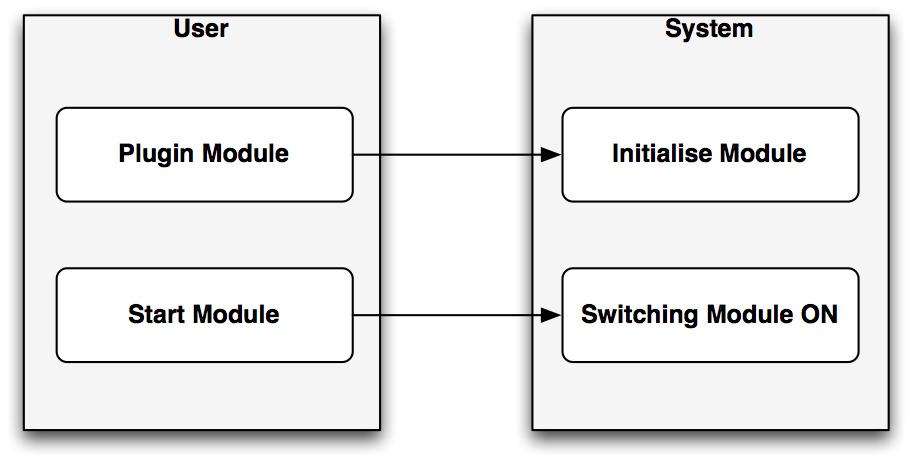
\includegraphics[width=0.8\textwidth]{images/sys_int.png}
		\caption{Example of \textit{on system user} interaction}
	\end{centering}
\end{figure}

\begin{figure}[H]
	\begin{centering}
		 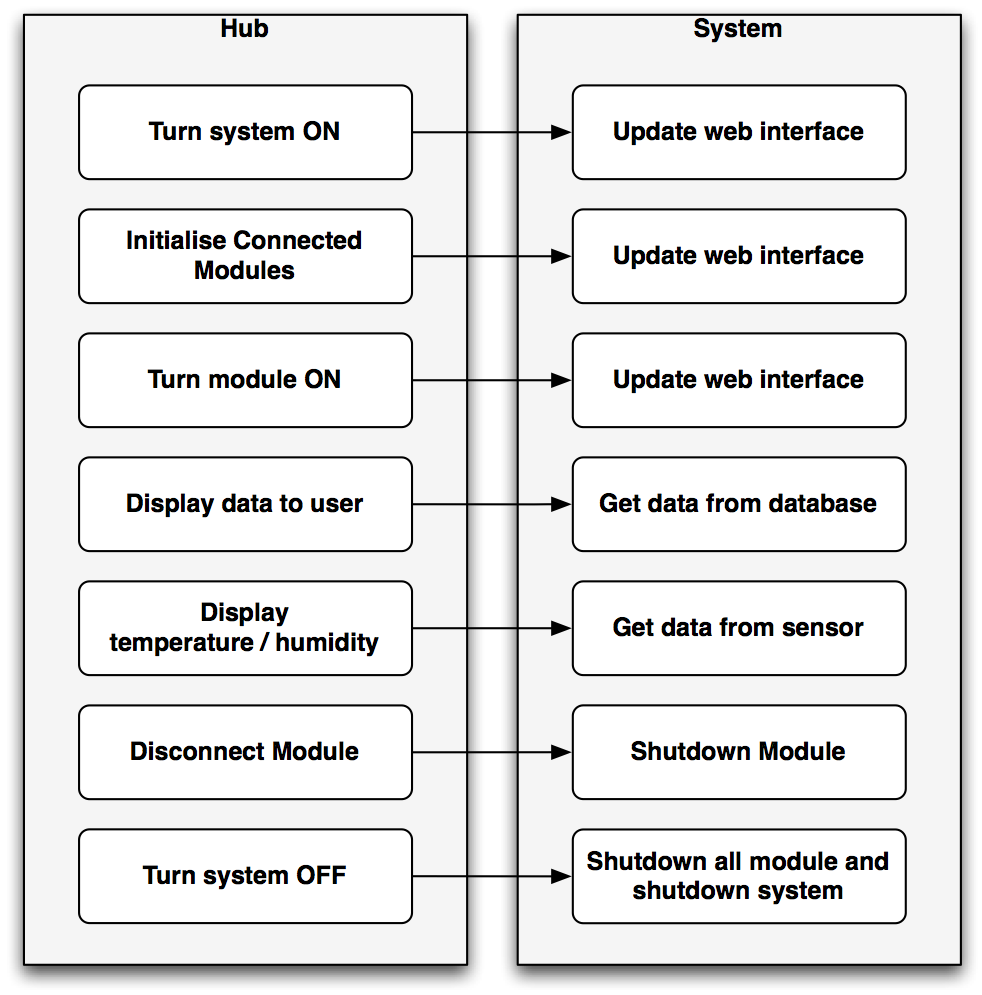
\includegraphics[width=0.8\textwidth]{images/hub_int.png}
		\caption{Example of \textit{hub} user interaction}
	\end{centering}
\end{figure}
	

%%%%%%%%%%%%%%%%%%%%%%%%%%%%%%%%%%%%%%%%%%%%%%%%%%%%%%%%%%
\subsection{Interface Analysis}
In the EIDE1 course the interaction design was made for the web interface and the physical interface for the hub, with different design sessions. The user needs and the design for the two interfaces was determined to be made. The IDE report is included in the appendix.
\begin{figure}[H]
	\begin{centering}
		 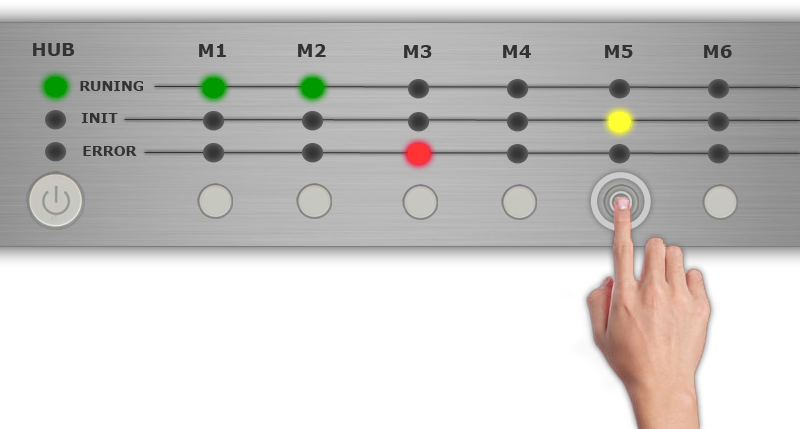
\includegraphics[width=0.75\textwidth]{images/hub_user_interact.png}
		\caption{Final design of the hubs physical interface.}
	\end{centering}
\end{figure}
\textbf{WebInterface:} In EWEB course a static web interface was developed with the knowledge gained from the interaction design sessions and developed in HTML, the WEB report is included in appendix.
\begin{figure}[H]
	\begin{centering}
		 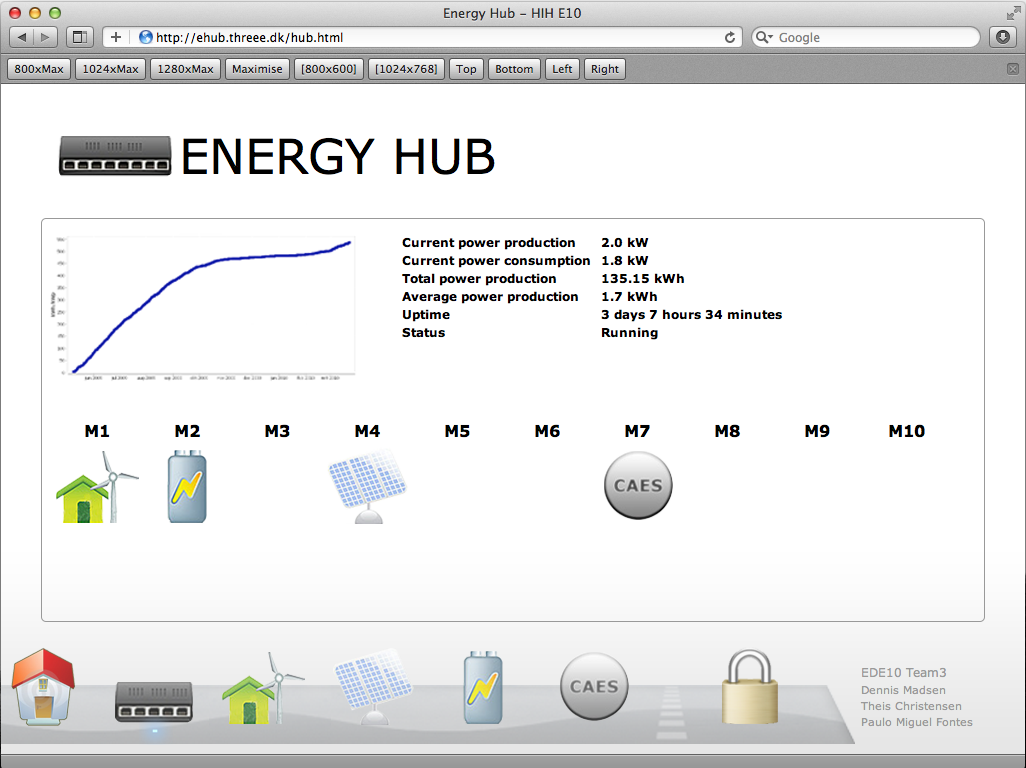
\includegraphics[width=0.69\textwidth]{images/screen_hub_page.png}
		\caption{The final web interface design, showing the hub module page}
 	\end{centering}
\end{figure}
\begin{figure}[H]
	\begin{centering}
		 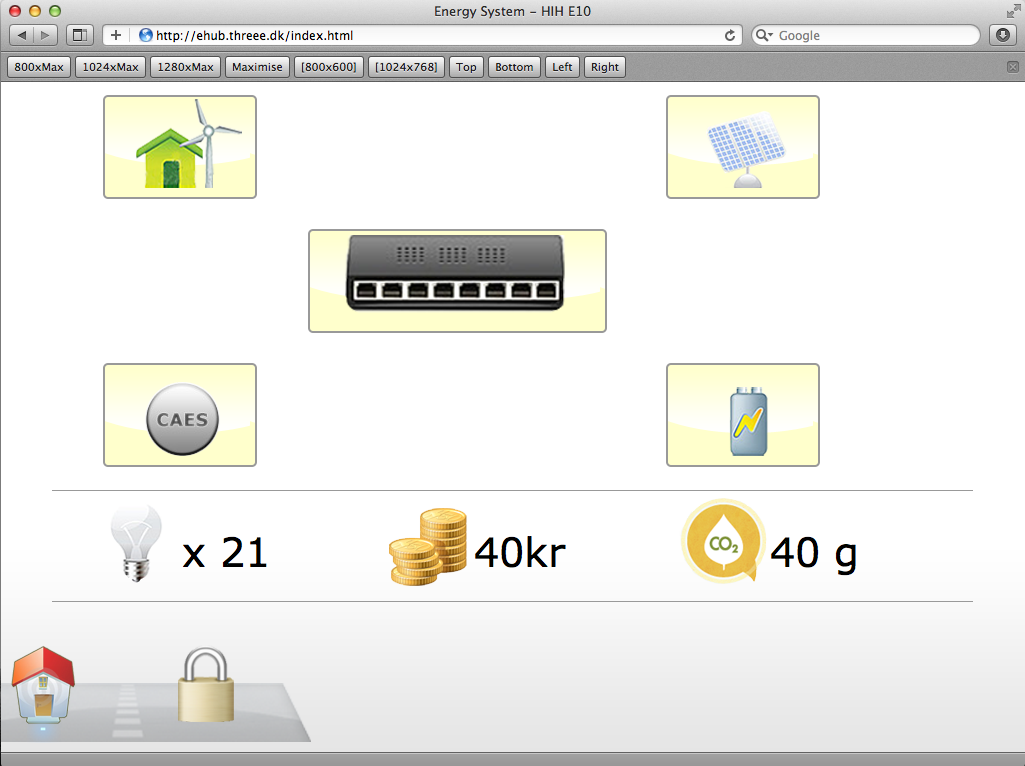
\includegraphics[width=0.69\textwidth]{images/screen_index_page.png}
		\caption{The final web interface design, showing index page}
 	\end{centering}
\end{figure}

%%%%%%%%%%%%%%%%%%%%%%%%%%%%%%%%%%%%%%%%%%%%%%%%%%%%%%%%%%
\subsection{Function Analysis}
From an analytic perspective, functions are very useful as they are intended to elaborate the objective of the system. When defining functions the question is, \textit{what is the system supposed to do?} In the usage part, it was concerned \textit{how} the system should be used. This makes the usage and functions closely connected, since it is difficult to talk about how a system is being used without discussing what it should do.
\\\\ When analyzing functions the object is to get a complete list of all the functions the system must implement. The goal is not to describe every single function in detail, quite the contrary the goal is to identify the functions.
\\\\ Functions can be grouped into types. There are four different types of functions:
\\\\ \textit{Update} is a type defining functions which are activated by a problem or application domain event, and which results in a change in the models state.
\\\\ The type \textit{Signal} defines a function which is triggered by a change in the models state. Running the function always results in a reaction to its surroundings: that is either the reaction is a display to the actors in the problem domain or else the reacting a direct intervention in the problem domain.
\\\\ When an actor has need for information the function of type \textit{Read} is activated. The function is displaying the relevant data of the model to the actor.
\\\\ Finally, the \textit{Calculating} function is activated when an actor provides information, which should be included in a computation which also involves data from the model. The function returns its computed result to a display.
\\\\ When all functions are found they must be defined by their type and complexity, as shown below.\\
\begin{table}[H]
	\begin{tabular}{| p{11cm} | p{2cm} | p{3cm} |}
	\hline
	\textbf{Title}								& \textbf{Complexity}	& \textbf{Type}		\\ \hline
	connect\_module							&&
	\\ Modules can be connected no the back of the hub	& S				& Update 			\\ \hline
	disconnect\_module							&&
	\\ Modules can be disconnected on the back of the hub & S			& Update	 		\\ \hline
	start\_system								&&
	\\ Start the hub from the physical interface			 & S				& Update 			\\ \hline
	stop\_system								&&
	\\ Stops all modules including the hub & S		& Update 			\\ \hline
	power\_off\_system							&&
	\\ Critical error, shut down it self				& S				& Update 			\\ \hline
	start\_module								&&
	\\ Modules can be started from the hubs web page & M				& Update 			\\ \hline
	initialize\_module							&&
	\\ Modules are automatically initialized when connected & C			& Update/Calculating\\ \hline
	stop\_module								&&
	\\ Modules can be stopped from the hubs web page	& M				& Update 			\\ \hline
	get\_module\_production						&&
	\\ Read data from module						& M				& Read/Calculating 	\\ \hline
	get\_module\_consumption					&&
	\\ Read data from module						& M				& Read/Calculating 	\\ \hline
	get\_module\_energy\_level					&&
	\\ Read data from module						& M				& Read/Calculating 	\\ \hline
	get\_temperature							&&
	\\ Read temperature sensor					& M				& Read/Calculating	\\ \hline
	get\_humidity								&&
	\\ Read humidity sensor						& M				& Read/Calculating	\\ \hline
	create\_module\_log	\_file 					&&
	\\ Create a log file for a module					& VC				& Read/Update		\\ \hline
	load\_module\_log	\_file 					&&
	\\ Load an already created log file of a module		& C				& Read/Update		\\ \hline
	save\_module\_log	\_file 					&&
	\\ Save a new log file of a module				& C				& Read/Update		\\ \hline
	send\_module\_command 					&&
	\\ Send a command to a module				& M				& Update			\\ \hline
	read\_module\_command 					&&
	\\ Read a command from a module				& M				& Read/Update		\\ \hline	
	webserver\_write\_data	 					&&
	\\ Write data to the web server					& M				& Update			\\ \hline	
	webserver\_read\_data 						&&
	\\ Read data from the web server				& M				& Read/Update		\\ \hline	
	\end{tabular}
	\caption{Table showing the different functions in the system. \\S = simple. M = medium. C = complex. VC = very complex}
	\label{Function_table}
\end{table}

%%%%%%%%%%%%%%%%%%%%%%%%%%%%%%%%%%%%%%%%%%%%%%%%%%%%%%%%%%
\subsection{System Dynamics}
Diagram of how to put data on the web server.
\begin{figure}[H]
	\begin{centering}
		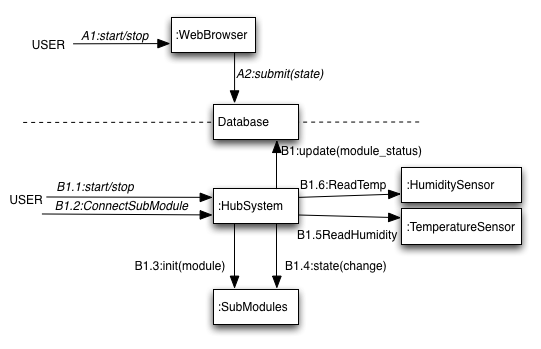
\includegraphics[width=0.7\textwidth]{images/communication_diagram.png}
		\caption{Interaction between systems; Web browser and Hub both connected to the database}
 	\end{centering}
\end{figure}		
\todo[inline]{MORE DIAGRAMS :D}

%%%%%%%%%%%%%%%%%%%%%%%%%%%%%%%%%%%%%%%%%%%%%%%%%%%%%%%%%%
%%%%%%%%%%%%%%%%%%%%%%%%%%%%%%%%%%%%%%%%%%%%%%%%%%%%%%%%%%
\section{General Architecture Design}
Design criteria is important to consider in order to choose the right technical platform to perform the criteria. When marketing the product design criteria is very important, in making the specification for the product.
%%%%%%%%%%%%%%%%%%%%%%%%%%%%%%%%%%%%%%%%%%%%%%%%%%%%%%%%%%
\subsection{Design Criteria}
Write in what parts should be used (mostly off the shelf things).
\begin{table}[H]
	\begin{tabular}{| r | c | c | c | c | c |}
	\hline
		Issue 					& Critical 	& Very Important 	& Important	& Less Important	& Notes \\ \hline
		Safe					& X 		& ~ 				& ~			& ~ 				& 1 \\ \hline
		Performance 			& ~			& ~ 				& X 		& ~ 				& 2 \\ \hline
		Usage 					& X 		& ~ 				& ~ 		& ~ 				& 3 \\ \hline
		Reliability 			& X 		& ~ 				& ~ 		& ~ 				& 4 \\ \hline
		Easy serviceable 		& ~ 		& X 				& ~ 		& ~ 				& 5 \\ \hline
		Remote maintenance 		& ~ 		& ~ 				& X 		& ~ 				& 6 \\ \hline
		Cost effective 			& ~ 		& ~ 				& ~ 		& X 				& 7 \\ \hline
		Learnability			& ~ 		& X 				& ~ 		& ~ 				& 8 \\ \hline
		Memorability			& ~ 		& X 				& ~ 		& ~ 				& 9 \\ \hline
		Effectiveness			& ~ 		& ~ 				& X 		& ~ 				& 10 \\ \hline
		Utility					& ~ 		& ~ 				& ~ 		& X 				& 11 \\ \hline
	\end{tabular}
	\end{table}
Notes:
\begin{enumerate}
	\item The safety is a very important factor, as the system is meant as a showoff system for high-school students, who should be able to be near the system without hurting themselves or the system.
	\item The performance in the system is not critical when considering it from the users perspective. It doesn't matter if it takes a few seconds before the system responds the user. But the system should still be able to react fast in order not to harm it self, but also to get a high effectiveness. 
	\item The system should be easy to use. All kinds of people should be able to use the system without any specific training. Connecting of new devices and doing administrative jobs on the system a small walk through of the system is required. 
	\item Errors must not occur in the system. The hub is the central nerve in the whole system, therefore if the hub does not run, non of the subsystems does and no energy is routed.
	\item The user of the system should be able to find eventual errors on the system by him self, with help from a good error log created by the system.
	\item The only thing possible to maintain remotely is start and stop of submodules + power down the whole system, which is less important as the system is placed locally.
	\item Only one kind of the system is to be produces, but still the price should be kept at a relatively low level (as we have an undefined maximum price of the system).
	\item As the system is meant to be operated by a non-technically persons, learning the system shall be fast and operating the system shall therefore be very intuitive. Also visitors should be able to do simple tasks on the system, such as turn a device on or off.
	\item Mainly the system is supposed to run by it self without any interaction. But when the system is going to be operated on, or the system is showed for visitors, the instructed person(s) shall be able to do so without any preparation time.
	\item The effectiveness of the system is not the most important factor, but still quite important as the talk is about a green system, which must be
	affordable for the user to implement the system. When investing in a green system, it will have information about estimated lifetime and buy time (the time it takes the system to `buy home itself'). If the buy time is to long, maybe longer than the lifetime, the price for having such a system will be way to high. The goal is that visitors can see the advantage in buying a green system (environmental and money friendly), so it might affect them to be more environmental friendly. 
	\item The possibility of changing parameters in the system should be kept as low as possible to easy the interaction with the system. If the user have too many ways of setting up the system it can easily confuse more than necessary. Therefore only the most important things that the user should be able to change is implemented, rest of the settings is placed as hidden utilities (only to be set up by the developers during tests). 
\end{enumerate}

%%%%%%%%%%%%%%%%%%%%%%%%%%%%%%%%%%%%%%%%%%%%%%%%%%%%%%%%%%
\subsection{Architecture Dynamics}
The sequence diagram explain the dynamics of more complex parts of the system, this diagram is important for estimating the price and time for the development, by giving the developer a better understanding of how the system works.

\begin{figure}[H]
	\begin{centering}
		 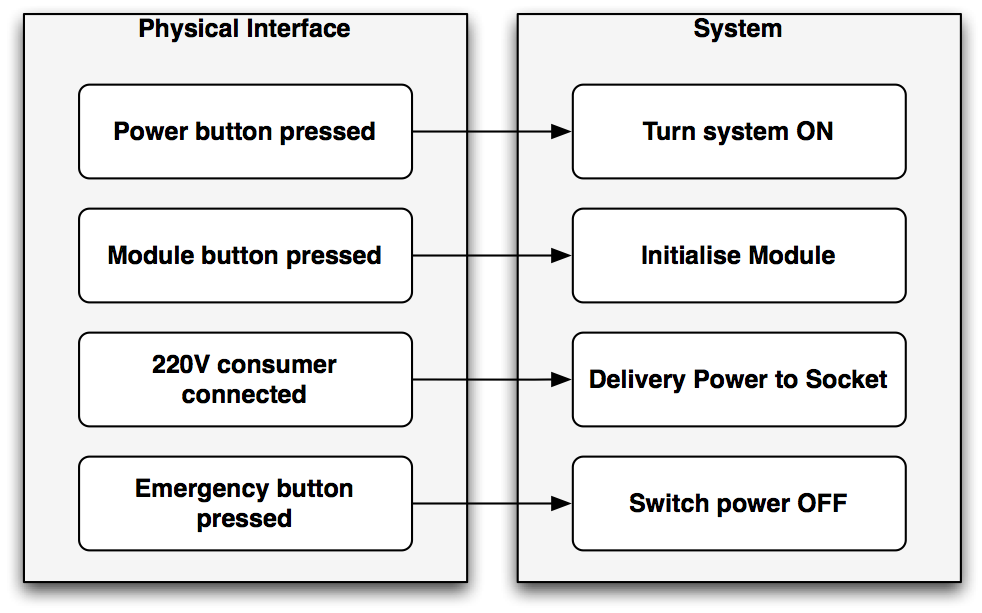
\includegraphics[width=0.8\textwidth]{images/phy_sys.png}
		\caption{Sequence diagram; Communication between the system and external systems.}
 	\end{centering}
\end{figure}

\textbf{Sequence Diagrams}
\begin{figure}[H]
	\begin{centering}
		 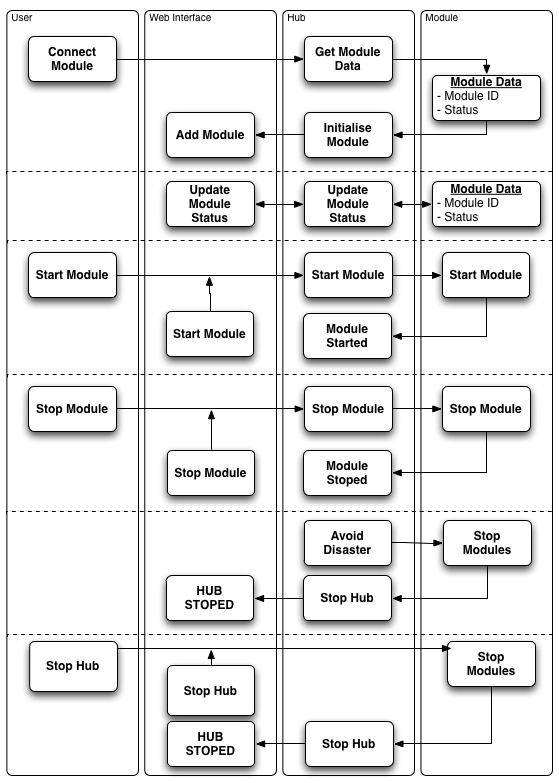
\includegraphics[width=0.8\textwidth]{images/SequenceDiagram.png}
		\caption{Sequence diagram; Communication between the system and external systems.}
 	\end{centering}
\end{figure}

%%%%%%%%%%%%%%%%%%%%%%%%%%%%%%%%%%%%%%%%%%%%%%%%%%%%%%%%%%
%%%%%%%%%%%%%%%%%%%%%%%%%%%%%%%%%%%%%%%%%%%%%%%%%%%%%%%%%%
\section{Technical Platform}
Selecting the technical platform is very important. The wrong platform may cause negative effects on the final product, or in the cost of the development of the product. The hardware have different specifications and lifetime. Here the design criteria is a big help for selecting the right platform, to fulfill the requirements
%%%%%%%%%%%%%%%%%%%%%%%%%%%%%%%%%%%%%%%%%%%%%%%%%%%%%%%%%%
\subsection{Hardware Specifications}
As hardware we are going to use the following:
\begin{itemize}
	\item Embedded Artists LPC2478-32 Developer kit.
	\item Temperature sensor
	\item Humidity sensor
	\item Current sensor
	\item Digital Converter
	\item Line communication module
\end{itemize}
%%%%%%%%%%%%%%%%%%%%%%%%%%%%%%%%%%%%%%%%%%%%%%%%%%%%%%%%%%
\subsection{Software Specifications}
In the software part we are using the ARM processor, and we have to develop drivers for the different hardware above, we are also making the following in software:
\begin{itemize}
	\item Web 
	\item Ethernet communication
	\item Storage module driver
	\item Producer module driver
	\item Consumer module driver
\end{itemize}
\begin{table}[H]
	\begin{center}
	\begin{tabular}{| p{5cm}  | p{2.5cm} | p{1cm} | p{1cm} |}
	\hline
		\textbf{Class}					& \textbf{Interface}	& \textbf{HW}	& \textbf{SW}	\\ \hline
		\textbf{System:}					&			&		&		\\ \hline
		ARM							& DIG		&		& X 		\\ \hline
		PLC module					& DIG/ANA	& X		& X 		\\ \hline
		Power switch					& DIG/ANA	& X		& X 		\\ \hline
		Digital Converter				& DIG/ANA	& X		& X 		\\ \hline
		Current sensor					& DIG/ANA	& X		& X 		\\ \hline
		\textbf{Sensor:}					&			&		&		\\ \hline
		Temperature					& ANA		& X		& 	 	\\ \hline
		Humidity						& ANA		& X		& 		\\ \hline
		\textbf{Web interface:}			&			&		&		\\ \hline
		Ethernet						& DIG		& 		& X	 	\\ \hline
		Web server					& DIG		& 		& X		\\ \hline
		\textbf{Other:}					&			&		&		\\ \hline
		Grid							& ANA		& X		& 	 	\\ \hline
		\textbf{Modules:}				&			&		&		\\ \hline
		Storage						& DIG		& 		& X	 	\\ \hline
		Producer						& DIG		& 		& X		\\ \hline
		Consumer					& DIG		& 		& X		\\ \hline
		\textbf{Physical interface:}			&			&		&		\\ \hline
		Interface						& DIG/ANA	& X		& X	 	\\ \hline
		Indicator						& DIG/ANA	& X		& X		\\ \hline
	\end{tabular}
	\caption{HW + SW Specifications. DIG = Digital. ANA = Analog. HW = Hardware. SW = Software}
	\end{center}
\end{table}

%%%%%%%%%%%%%%%%%%%%%%%%%%%%%%%%%%%%%%%%%%%%%%%%%%%%%%%%%%
%%%%%%%%%%%%%%%%%%%%%%%%%%%%%%%%%%%%%%%%%%%%%%%%%%%%%%%%%%
\section{Contracting}
\begin{table}[H]
	\begin{tabular}{| p{1cm} |p{5cm}|p{10cm}|}
		\hline
		Week&	Task					&			Note 						\\\hline
		5 	& 							&	EMC course, Meeting with MOJ and KK	\\\hline
		6	& 							&				 						\\\hline
		7	& 							&	Meeting with MOJ and KK			 	\\\hline
		8	& 							&				 						\\\hline
		9	& 							&	Meeting with MOJ and KK			 	\\\hline
		10	& 							&				 						\\\hline
		11	& 							&	Meeting with MOJ and KK			 	\\\hline
		12	& 							&				 						\\\hline
		13	& 							&	Meeting with MOJ and KK, Project week\\\hline
		14	& 							&	Easter holiday					 	\\\hline
		15	& 							&	Meeting with MOJ and KK			 	\\\hline
		16	& 							&				 						\\\hline
		17	& 							&	Meeting with MOJ and KK			 	\\\hline
		18	& 							&				 						\\\hline
		19	& 							&	Meeting with MOJ and KK			 	\\\hline
		20	& 							&	Project week			 			\\\hline
		21	& 							&	Meeting with MOJ and KK, Project week, submit project \\\hline
	\end{tabular}
	\caption{Time plan for 4. semester}
\end{table}
